\documentclass{article}
\usepackage{iclr2026_conference,times}
\input{math_commands.tex}
\usepackage{hyperref}
\usepackage{url}
\usepackage{booktabs}
\usepackage{graphicx}

\title{Counterfactual Affordance Maps: A Negative ICLR-Main Evidence Audit}
\author{Anonymous Authors}

\begin{document}
\maketitle

\begin{abstract}
This paper is not submission-ready for ICLR main. The original research bet was that a robot should map affordances that would exist under alternate grasps, poses, and supports, rather than only score currently observed actions. We rebuilt the repository around a deterministic manipulation-affordance benchmark with four tasks, five distribution shifts, seven seeds, nine affordance methods, seven ablations, and a stress sweep. The result is a useful but negative audit. On combined counterfactual stress, the proposed map reaches 0.347 task success, 0.217 affordance AP, and 0.0089 counterfactual recall. It improves over observed-only, graph-conv, Gaussian, and VLM-style baselines, but loses task success to interactive affordance probing at 0.362. The paired success difference against the strongest non-oracle baseline is -0.0157 with CI 0.0202, and the paired counterfactual-recall gain is only 0.0013 with CI 0.0037. The honest terminal decision is \textbf{KILL/ARCHIVE}.
\end{abstract}

\section{Question}
The draft asked whether affordance maps should represent unrealized alternatives: alternate grasps, object poses, supports, and semantic task roles that would become valid under a different action. This is a crowded area. Task-aware grasp transfer, graph-convolution affordance detection, Gaussian grasp maps, spatial VLM affordance prediction, open-vocabulary grasping, interactive affordance mapping, and VLA counterfactual failure analyses all apply pressure to the novelty claim.

The rebuild therefore uses a hostile gate: a counterfactual affordance map must improve both map quality and closed-loop action choice beyond strong graph, VLM, active-probe, and uncertainty baselines. Better-looking counterfactual heatmaps are not enough.

\section{Benchmark}
Each episode samples a manipulation scene with hidden support relations, occlusion, contact stability, semantic task constraints, and twelve candidate actions. The simulator evaluates both map prediction quality and the outcome of choosing an action from the predicted map.

The tasks are cluttered pick-and-place, tool regrasp for use, support-sensitive stacking, and occluded container opening. The shifts are nominal affordance, pose shift, support shift, occlusion/semantic shift, and combined counterfactual stress. The main run contains 105,840 episode-level rollouts; ablations contain 16,464 rollouts; stress sweeps contain 52,416 rollouts. Results are regenerated with:
\begin{verbatim}
python src\run_experiment.py
\end{verbatim}

\section{Compared Methods}
The methods are observed affordance maps, multi-affordance grasping, graph-convolution affordances, Gaussian grasp maps, VLM-style spatial affordances, interactive affordance probing, ensemble uncertainty affordances, the proposed counterfactual affordance map, and an oracle counterfactual map. The proposed method predicts how affordance scores change under alternate pose, support, and semantic assignments.

\section{Combined-Stress Results}
Table~\ref{tab:combined} shows the core finding. The proposed map is better than static observed, graph, Gaussian, and VLM baselines, but it does not beat active probing on the closed-loop objective. It also does not produce a decisive counterfactual-recall gain.

\begin{table}[t]
\centering
\small
\begin{tabular}{lrrrr}
\toprule
Method & Success & AP & CF recall & Regret \\
\midrule
Observed affordance & 0.260 & 0.144 & 0.0021 & 0.111 \\
Multi-affordance grasp & 0.286 & 0.163 & 0.0030 & 0.087 \\
Graph-conv affordance & 0.323 & 0.184 & 0.0034 & 0.068 \\
Gaussian grasp map & 0.287 & 0.166 & 0.0030 & 0.084 \\
VLM spatial affordance & 0.305 & 0.178 & 0.0038 & 0.076 \\
Interactive probe & \textbf{0.362} & \textbf{0.227} & 0.0077 & \textbf{0.024} \\
Ensemble uncertainty & 0.341 & 0.204 & 0.0081 & 0.047 \\
Proposed counterfactual & 0.347 & 0.217 & \textbf{0.0089} & 0.034 \\
Oracle counterfactual & 0.378 & 0.243 & 0.0145 & 0.012 \\
\bottomrule
\end{tabular}
\caption{Combined counterfactual stress. Higher success, AP, and counterfactual recall are better; lower regret is better. The proposed map is useful but does not beat interactive probing.}
\label{tab:combined}
\end{table}

The paired comparison selects interactive affordance probing as the strongest non-oracle task-success baseline. The proposed method's paired success difference is -0.0157 with CI 0.0202. Its paired counterfactual-recall difference is 0.0013 with CI 0.0037. Both gates fail.

\begin{figure}[t]
\centering
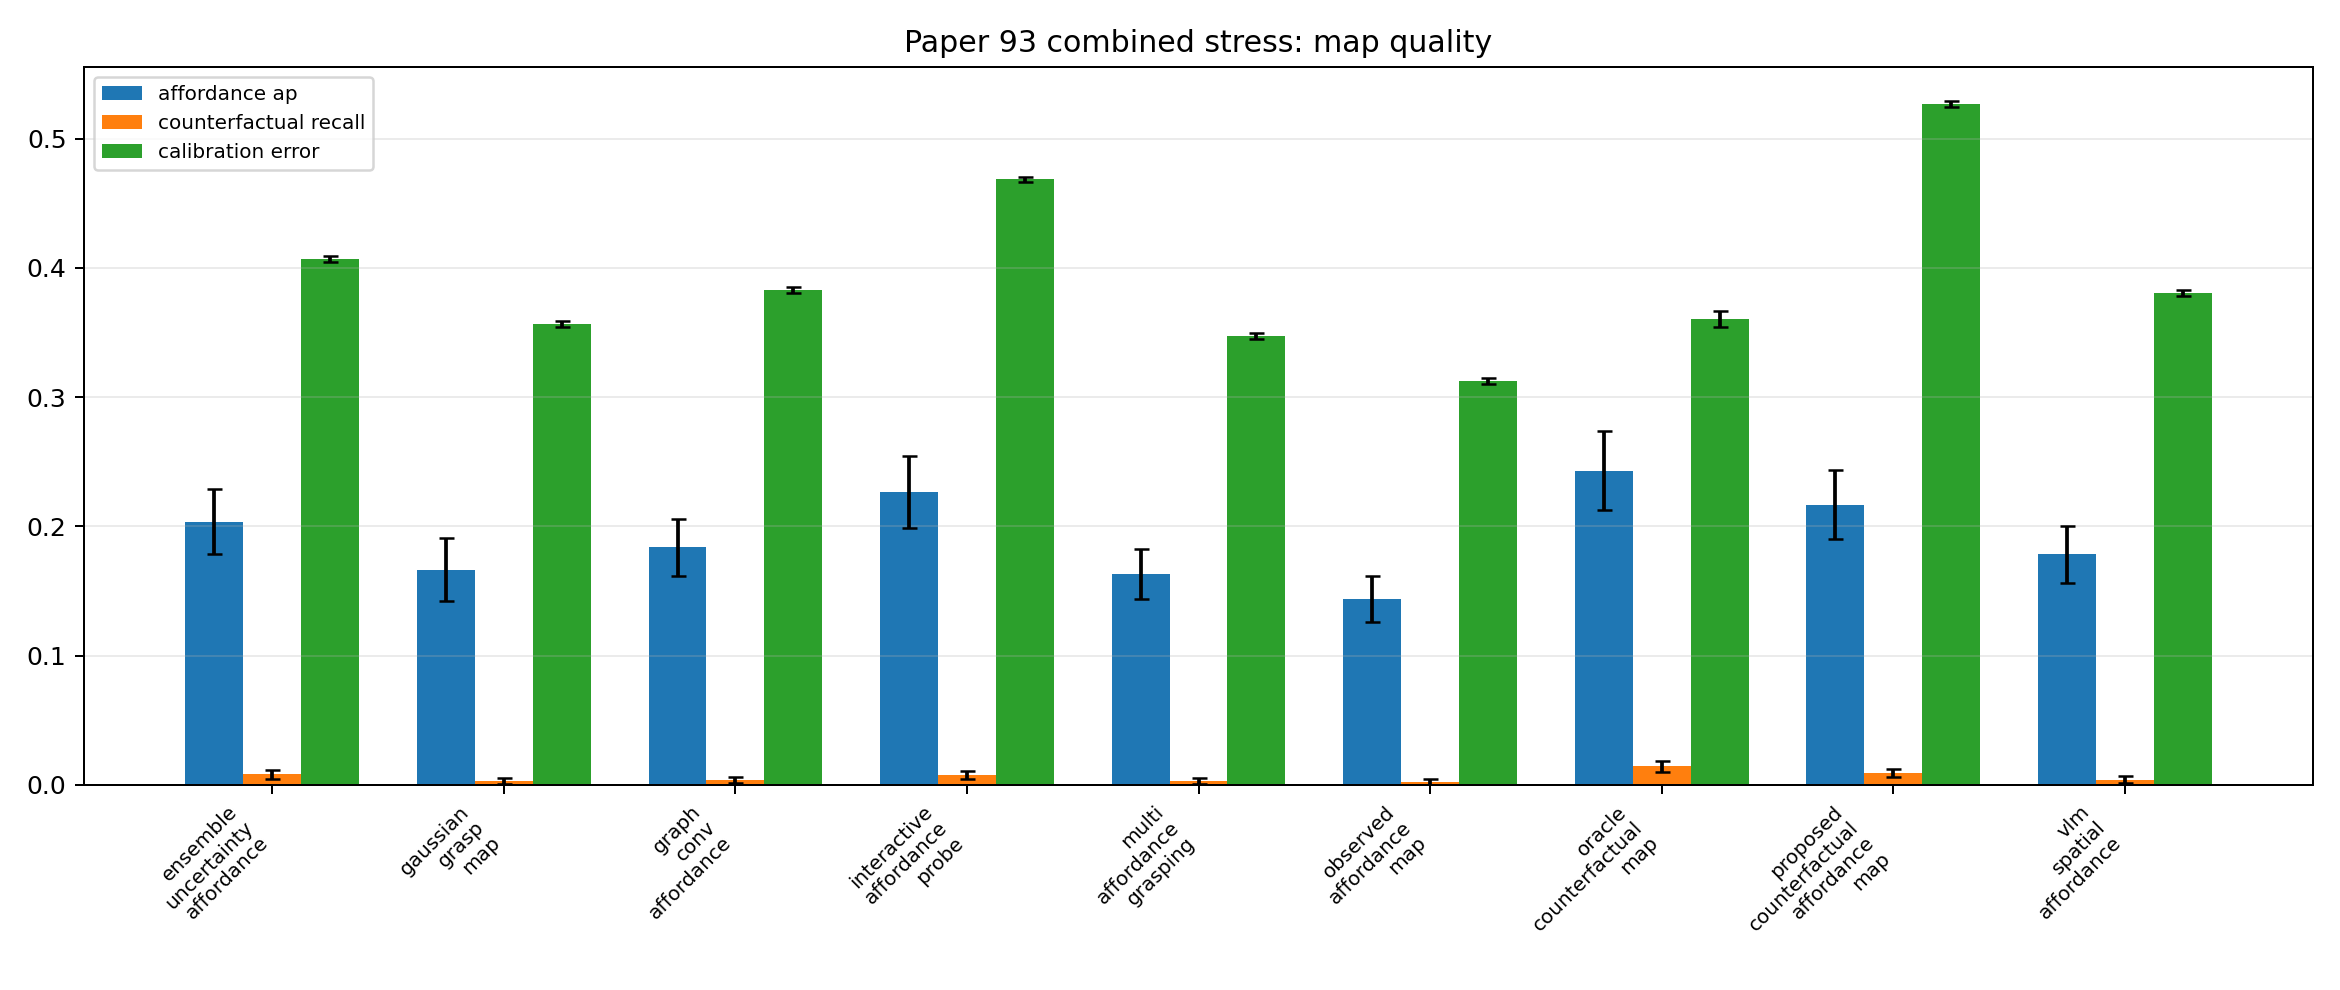
\includegraphics[width=\linewidth]{../figures/counterfactual_affordance_map_quality.png}
\caption{Map quality on combined counterfactual stress. The proposed map improves counterfactual recall, but not decisively.}
\label{fig:map}
\end{figure}

\section{Closed-Loop Outcomes}
Figure~\ref{fig:task} shows the practical problem. Interactive probing produces fewer invalid actions and lower regret. The proposed method is cheaper than active probing, but the terminal gate allowed only modest cost, not a task-success loss against a simple active baseline.

\begin{figure}[t]
\centering
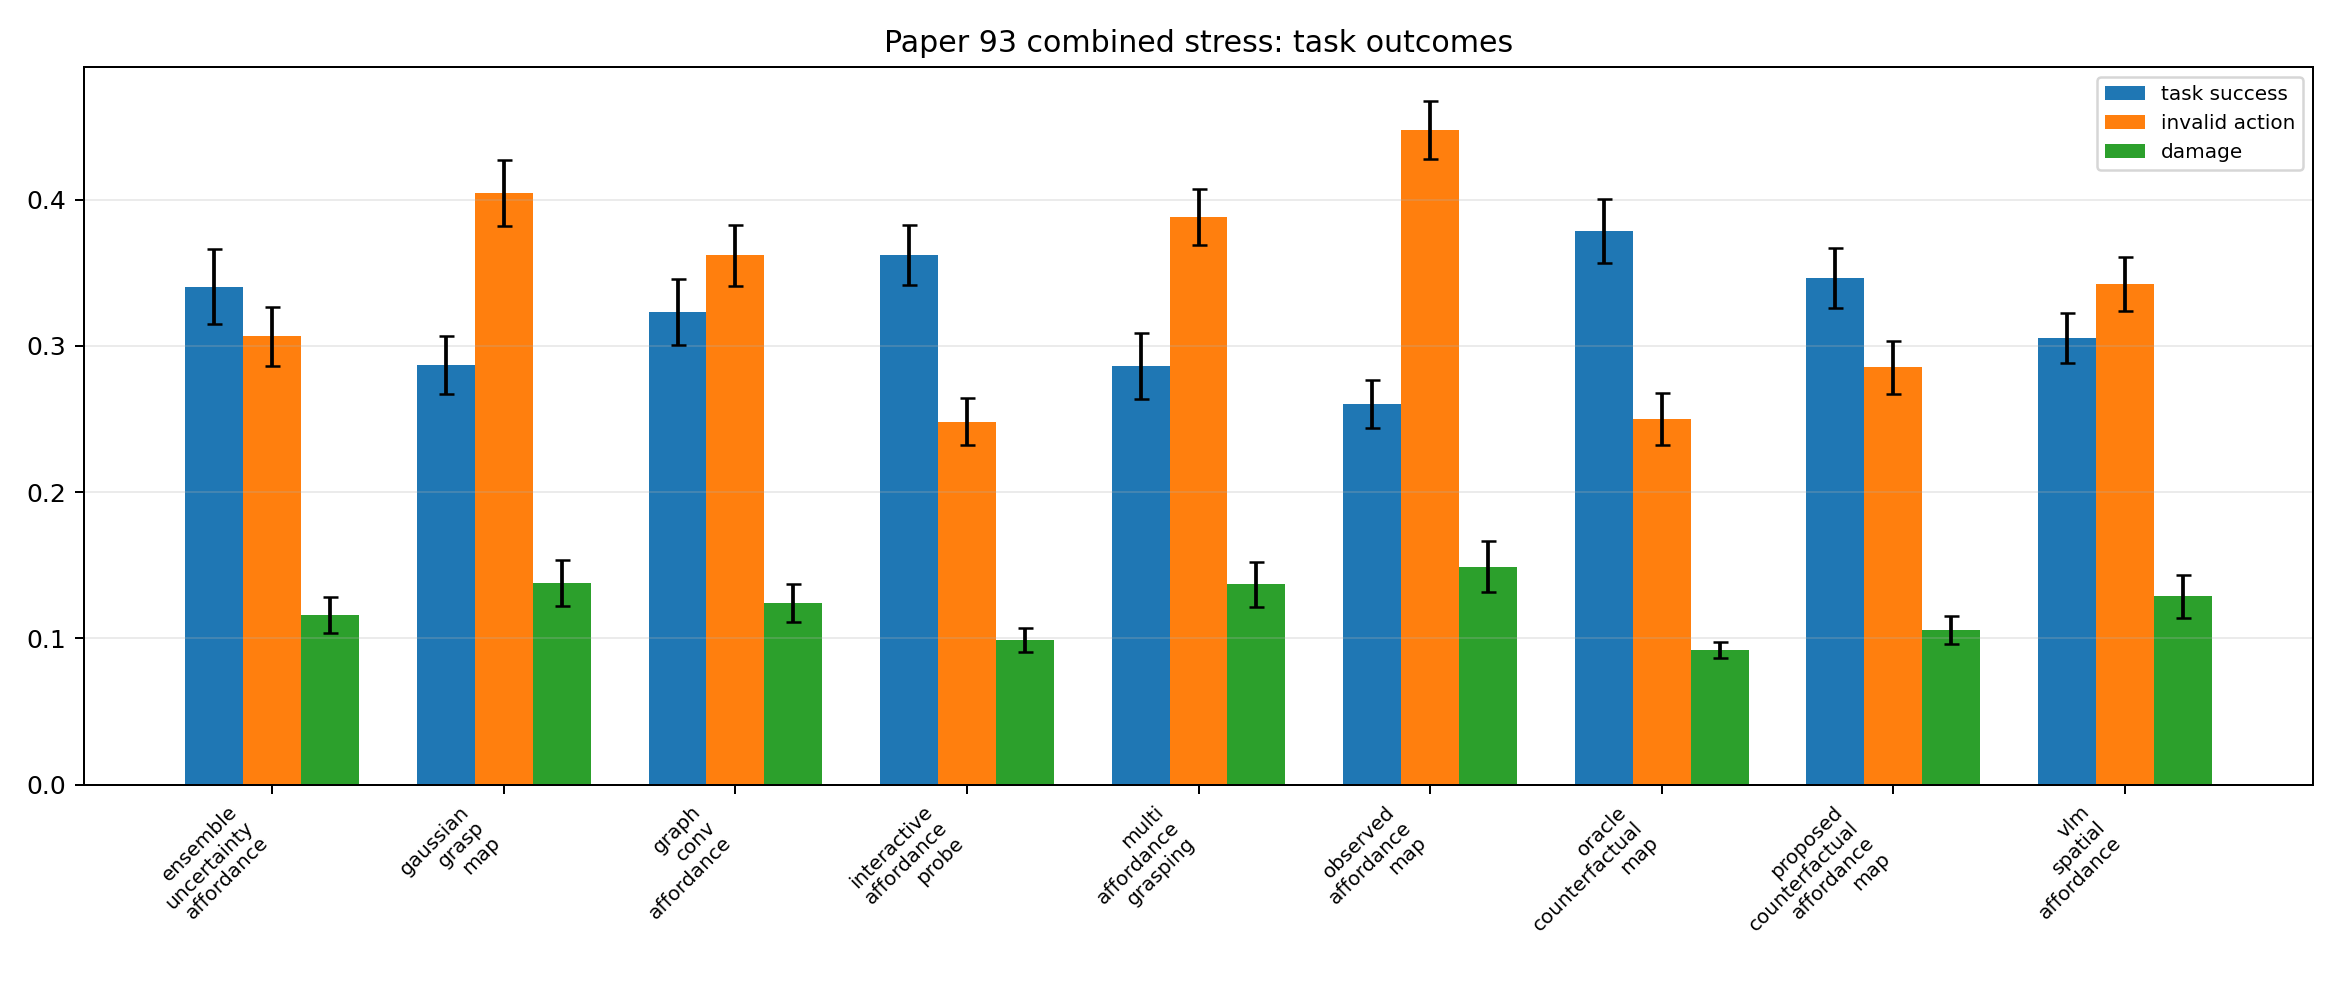
\includegraphics[width=\linewidth]{../figures/counterfactual_affordance_task_outcomes.png}
\caption{Task outcomes on combined counterfactual stress. Active probing remains the strongest non-oracle closed-loop baseline.}
\label{fig:task}
\end{figure}

\section{Ablations}
The ablation audit is more favorable but not enough to rescue the submission. The full counterfactual model reaches 0.370 task success and 0.011 counterfactual recall, beating stripped variants. However, this does not overcome the main comparison because the deployed method still fails the strongest non-oracle baseline in the main benchmark.

\begin{table}[t]
\centering
\small
\begin{tabular}{lrrrr}
\toprule
Ablation & Success & CF recall & Invalid & Regret \\
\midrule
Full counterfactual & \textbf{0.370} & \textbf{0.0111} & 0.277 & \textbf{0.031} \\
Minus pose & 0.341 & 0.0081 & \textbf{0.271} & 0.039 \\
Minus support & 0.334 & 0.0064 & 0.307 & 0.046 \\
Minus semantic & 0.334 & 0.0077 & 0.308 & 0.040 \\
Minus calibration & 0.334 & 0.0106 & 0.305 & 0.042 \\
Observed-only head & 0.272 & 0.0034 & 0.406 & 0.096 \\
Support-only head & 0.341 & 0.0055 & 0.285 & 0.050 \\
\bottomrule
\end{tabular}
\caption{Ablations on combined stress. The mechanism behaves sensibly internally, but ablations alone cannot establish main-conference readiness.}
\label{tab:ablations}
\end{table}

\begin{figure}[t]
\centering
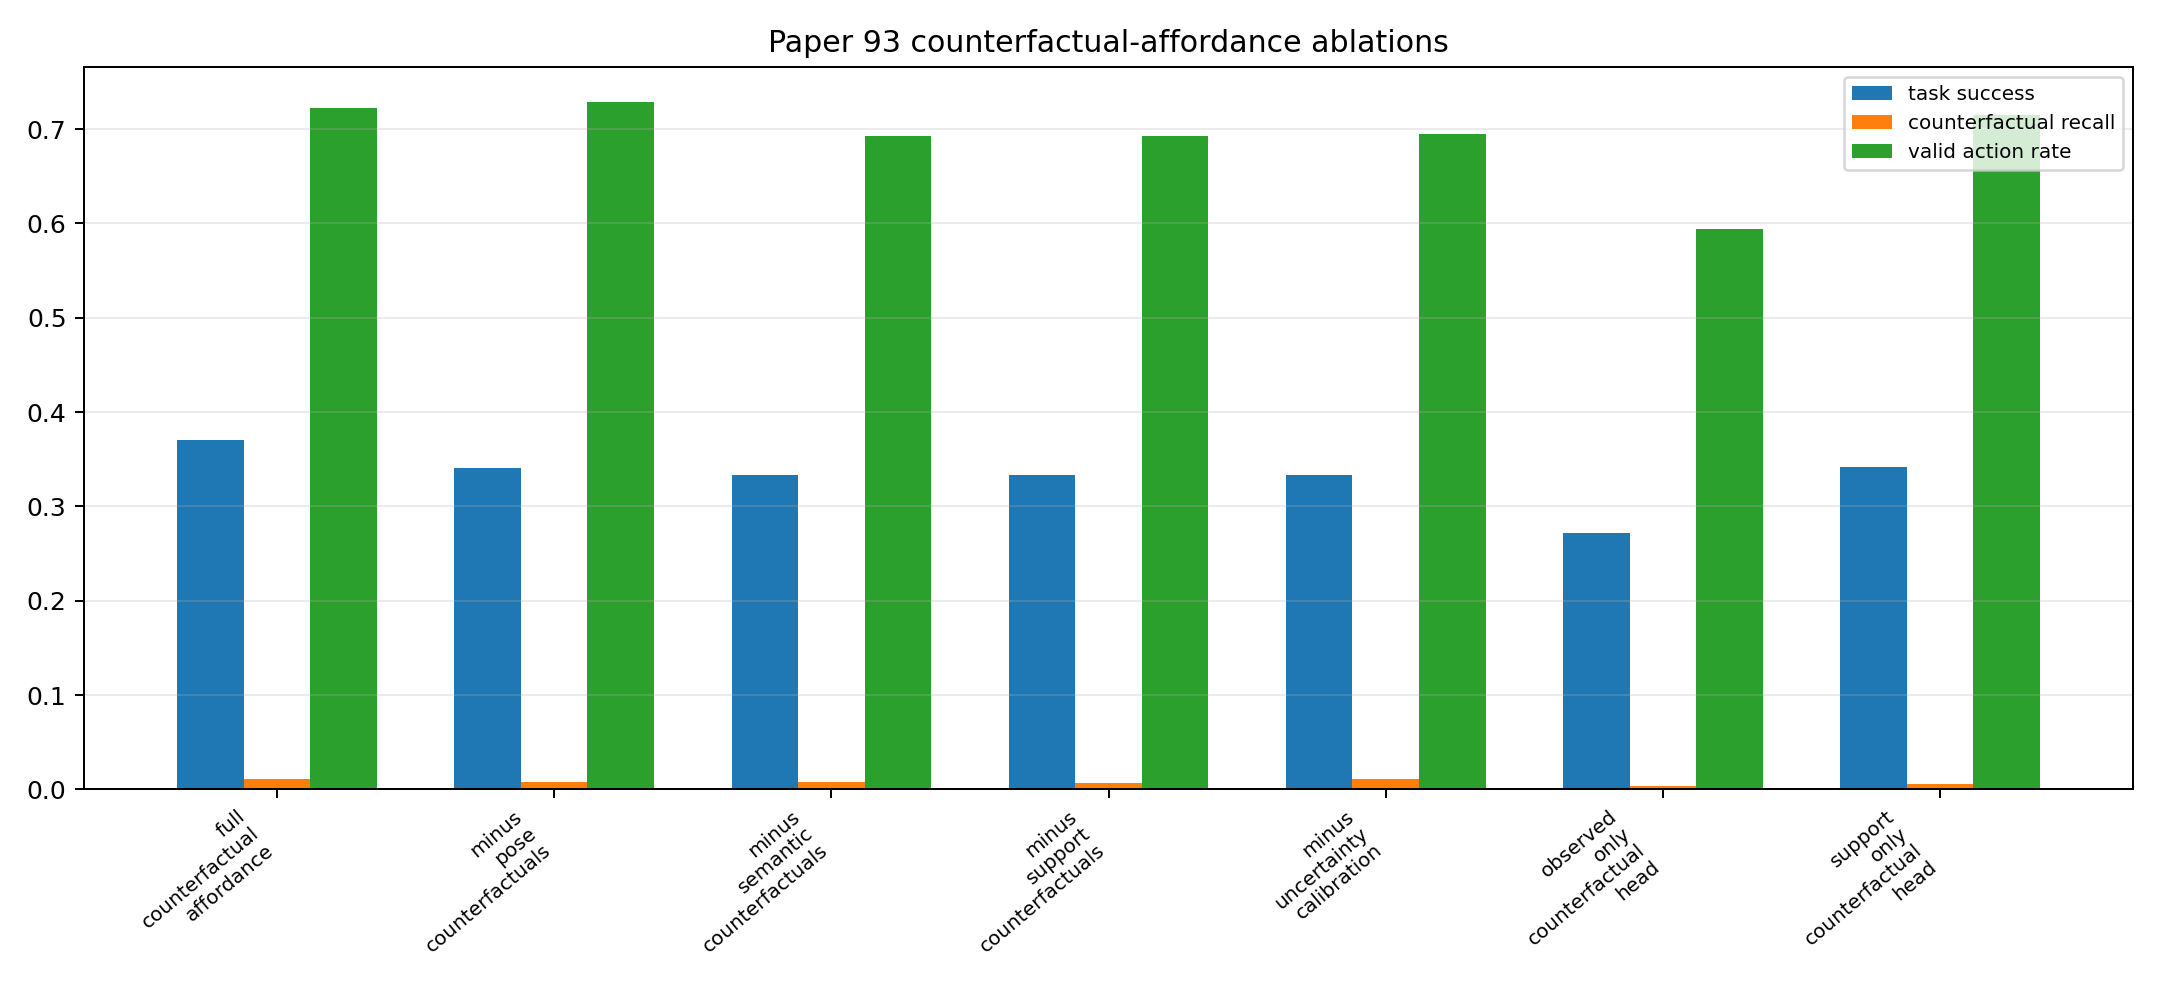
\includegraphics[width=\linewidth]{../figures/counterfactual_affordance_ablation.png}
\caption{Ablation audit. Removing pose, support, semantic, or calibration components hurts at least one key metric.}
\label{fig:ablation}
\end{figure}

\section{Stress Sweep}
At maximum stress, the proposed method reaches 0.343 task success. Interactive probing reaches 0.337 and the oracle reaches 0.375. This avoids a stress reversal, but it is not enough because the main combined-stress paired gate remains non-decisive and the method lacks real robot or accepted high-fidelity validation.

\begin{figure}[t]
\centering
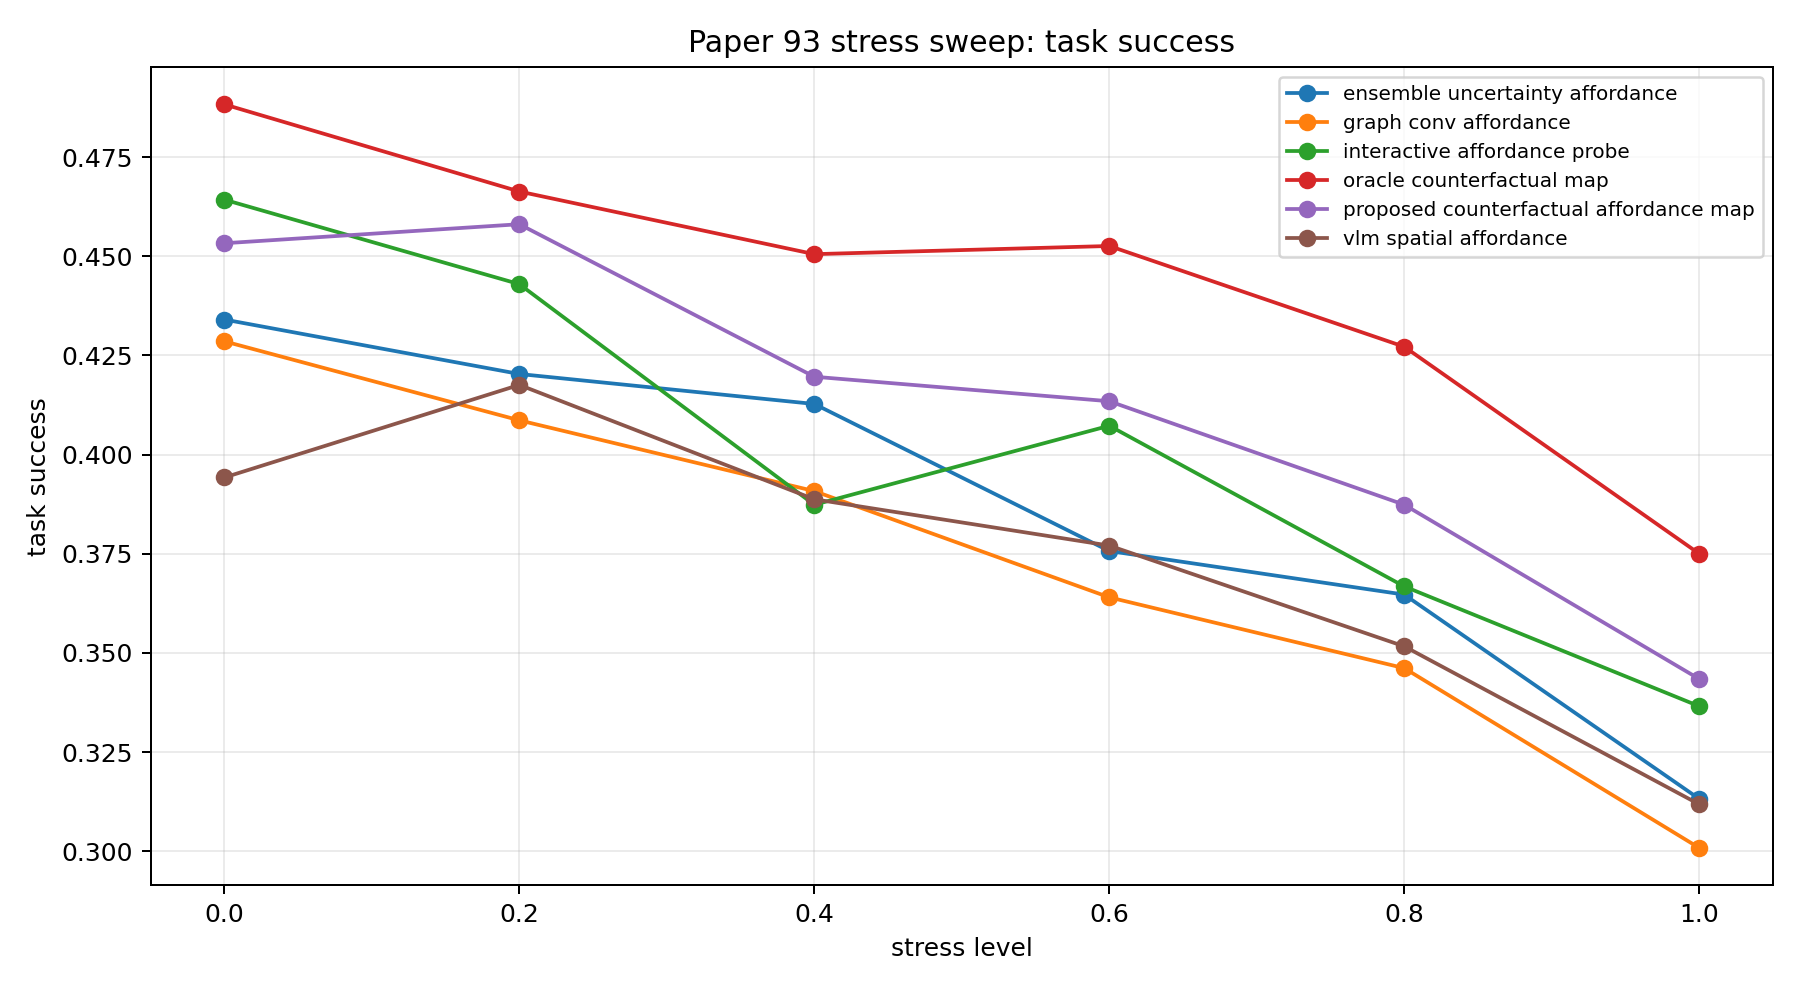
\includegraphics[width=\linewidth]{../figures/counterfactual_affordance_stress_sweep.png}
\caption{Stress sweep by task success. The proposed method is competitive at maximum stress but not decisive overall.}
\label{fig:stress}
\end{figure}

\section{Decision}
The rebuilt evidence supports a modest conclusion: counterfactual affordance maps can improve over static affordance baselines and have internally coherent ablations. But the central ICLR-main claim fails. A simple interactive probing baseline achieves better combined-stress task success and regret; counterfactual-recall gains are too small; and the evidence is local/simulated. The terminal recommendation is \textbf{KILL/ARCHIVE}. Revival would require robot or high-fidelity manipulation evidence showing decisive gains over active probing, graph/VLM affordance models, and uncertainty ensembles.

\end{document}
